% 原卷第6题的正弦曲线及标注；依图重绘，曲线按函数形式绘出，非截图。
\begin{tikzpicture}[x=1.35cm,y=0.72cm,line cap=round,line join=round]
  \draw[->] (-0.38,0) -- (3.45,0) node[right] {$x$};
  \draw[->] (0,-2.25) -- (0,2.25) node[above] {$y$};
  \draw[thick,domain=-0.34:3.32,samples=140,smooth,variable=\t]
    plot (\t,{2*sin(2*\t r+30)});
  \draw (-0.06,1) -- (0.06,1);
  \node[left] at (-0.06,1) {$1$};
  \node[below left] at (0,0) {$O$};
  \node[below] at (2.879793,0) {$\dfrac{11\pi}{12}$};
\end{tikzpicture}
